%%% LaTeX Template: Article/Thesis/etc. with colored headings and special fonts
%%%
%%% Source: http://www.howtotex.com/
%%% Feel free to distribute this template, but please keep to referral to http://www.howtotex.com/ here.
%%% February 2011
%%%
%%% Last updated September 2021 by CDM

%%%  Preamble
\documentclass[11pt,letterpaper]{article}
\usepackage[margin=1.0in]{geometry}
\usepackage[T1]{fontenc}
\usepackage[bitstream-charter]{mathdesign}
\usepackage[latin1]{inputenc}					
\usepackage{amsmath}						
\usepackage{xcolor}
\usepackage{cite}https://www.overleaf.com/project/631b8af69f1ea6c375d502b0
\usepackage{hyphenat}
\usepackage{graphicx}
\usepackage{float}
\usepackage{subfigure}
\usepackage{sectsty}
\usepackage[compact]{titlesec} 
\usepackage[tablegrid]{vhistory}
\allsectionsfont{\color{accentcolor}\scshape\selectfont}

%%% Definitions
\definecolor{accentcolor}{rgb}{0.0,0.0,0.5} 
\newcommand{\teamname}{Team UR5}
\newcommand{\productname}{Checkers-Playing UR5 Co-bot}
\newcommand{\coursename}{CSE 4316: Senior Design I}
\newcommand{\semester}{Fall 2022}
\newcommand{\docname}{Project Charter}
\newcommand{\department}{Department of Computer Science \& Engineering}
\newcommand{\university}{The University of Texas at Arlington}
\newcommand{\authors}{Nimita Uprety \\ Patricia Rojas \\ Hoang Ho \\ Kevin Vu \\ Joanna Huynh}

%%% Headers and footers
\usepackage{fancyhdr}
	\pagestyle{fancy}						% Enabling the custom headers/footers
\usepackage{lastpage}	
	% Header (empty)
	\lhead{}
	\chead{}
	\rhead{}
	% Footer
	\lfoot{\footnotesize \teamname \ - \semester}
	\cfoot{}
	\rfoot{\footnotesize page \thepage\ of \pageref{LastPage}}	% "Page 1 of 2"
	\renewcommand{\headrulewidth}{0.0pt}
	\renewcommand{\footrulewidth}{0.4pt}

%%% Change the abstract environment
\usepackage[runin]{abstract}			% runin option for a run-in title
%\setlength\absleftindent{30pt}			% left margin
%\setlength\absrightindent{30pt}		% right margin
\abslabeldelim{\quad}	
\setlength{\abstitleskip}{-10pt}
\renewcommand{\abstractname}{}
\renewcommand{\abstracttextfont}{\color{accentcolor} \small \slshape}	% slanted text

%%% Start of the document
\begin{document}

%%% Cover sheet
{\centering \huge \color{accentcolor} \sc \textbf{\department \\ \university} \par}
\vspace{1 in}
{\centering \huge \color{accentcolor} \sc \textbf{\docname \\ \coursename \\ \semester} \par}
% \vspace{0.5 in}
\begin{figure}[h!]
	\centering
   	
\includegraphics[width=0.5\textwidth]{images/Draft-Logo.png}
\end{figure}
% \vspace{0.5 in}
{\centering \huge \color{accentcolor} \sc \textbf{\teamname \\ \productname} \par}
\vspace{0.25 in}
{\centering \large \sc \textbf{\authors} \par}
\newpage


%\vspace{1 in}
%\centerline{January 13th, 2012}
%\newpage

%%% Revision History
\begin{versionhistory}
  	\vhEntry{0.1}{09.09.2022}{HH}{document creation}
  	\vhEntry{0.2}{10.03.2022}{NU, HH, PR, KV, JH}{complete draft}
 	\vhEntry{1.0}{10.03.2022}{NU, HH, PR, KV, JH}{release candidate 1}
 	\vhEntry{1.1}{04.28.2023}{KV, JH}{final revisions}
 	\vhEntry{2.0}{05.10.2023}{NU, HH, PR, KV, JH}{final revisions}
%  	\vhEntry{1.1}{10.31.2021}{AL}{added customer change requests *NEED TO EDIT}
\end{versionhistory}
\newpage

%%% Table of contents
\tableofcontents
\newpage

%%% List of figures and tables (optional)
\listoffigures
%\listoftables
\newpage
\setcounter{table}{0}

%%% Executive summary sections
\section{Problem Statement}
The UR5 collaborative robot (co-bot) belonging to the Computer Science department at the University of Texas at Arlington currently does not showcase the collaborative nature of its ability to interact closely with humans. The UR5 co-bot will be programmed to perform a complete game of the strategy board game, checkers, against a human opponent. The purpose of the UR5 co-bot project is to use the programmed co-bot as a marketing strategy for UT Arlington to expose students to industrial automation technology, introduce students to the UT Arlington College of Engineering and Computer Science Engineering departments, and provide an enjoyable educational experience. 

%The problem statement defines the "Why" of the project. This is the higher purpose, or the reason for the project's existence. This section should avoid mentioning implementation details, and focus more on what the current problem is and what would be gained if the problem were to be solved. In short, the is the reason that you are going to be working on something, not the method(s) that you will be employing.
\section{Methodology}
% This is the "What" of the project and it states what will be done to address the problem statement. This section should focus mostly on what your solution is going to be and what it is going to do (i.e., we are going to build an app, robot, device, etc. to perform some task which mitigates the problem). If someone were to ask you \textit{"What are you doing for your senior design project?"}, this is section is basically what you would tell them.

Our project's objective is to program the UR5 co-bot to play checkers against a human opponent. We aim to accomplish this by utilizing computer vision to analyze the current state of the board so that the co-bot can then make an educated choice as to which move to play next. In order to pick up each individual piece we will create an accessory that we will attach to the UR5 arm so that the checkers pieces can either be picked up by vacuum suction or through electropermanent magnetism. The robot and the human player will take turns moving pieces until one of them wins.

\section{Value Proposition}
With the UR5 co-bot's ability to play a game of checkers against a human opponent, our customer, Dr. Christopher McMurrough, will be able to present the robot arm to students for marketing and educational purposes. This is possible because the robot arm is safe, flexible, and interactive. Collaborative demonstrations with the arm may garner students' interest in STEM and in the University of Texas at Arlington. In addition to this, students will gain exposure to different projects that computer science, software engineering, and computer engineering students get to work with. Lastly, any profit made from the project through demonstrations can open opportunities for involvement with charity and donations.


% The Value Proposition explains how the sponsors will benefit from your work, and why they should invest funding, time, and expertise in supporting your team. Here, you are essentially making a case for the project. There are many ways in which value can be returned to your stakeholders (industrial sponsors, instructors, the university, etc.), list any that may help you convince them to "buy in".
\section{Development Milestones}
These are the milestones and completion dates for the project:
\begin{itemize}
  \item Project Charter first draft - October 2022
  \item System Requirements Specification - October 2022
  \item Architectural Design Specification - November 2022
  \item Demonstration of Gripper with Suction Cup - December 2022
  \item Detailed Design Specification - February 2023
  \item Demonstration of Robot Object Detection - February 2023
  \item Demonstration of Computer Vision Integration - March 2023
  \item CoE Innovation Day poster presentation - April 2023
  \item Demonstration of Robot Playing Checkers - April 2023
  \item Final Project Demonstration - May 2023
\end{itemize}
\newpage

%%% Remaining project charter sections
\section{Background}
% An in-depth explanation of the problem, including the "business case". What is wrong with the status-quo or what opportunity exists that justifies undertaking this project (expanding upon the problem statement)? If you have a clear customer or sponsor, why do they want you to work on this? What is the existing relationship, if any, between the development team and the customer? This section should occupy 1/2 - 1 full page.

Today, we live in an age of rapid technological advancements and increasing usages of mechanical and digital automation. Time and time again, modern technology has continued to showcase how it can be utilized to enrich the human experience. However, in order to continue advancing our technologies, we must pique the interest and inspire a new generation of innovators and engineers. In order to inspire this new generation, we can show them how we can apply new modern technologies to enrich existing familiar experiences.

Our project aims to showcase how a robot arm can be programmed to play a game of checkers, a game very familiar to many. Although there is no real need or demand for a checkers-playing robot today, there is a very real and growing demand for engineers in the modern world, especially when it comes to computing technologies. With this project, we hope to ignite new and existing passions for technology and innovation.

This isn't to say something similar to this hasn't been done before. There have been many projects in the past that involve a robot completing familiar tasks. Whether it be cooking dishes, brewing coffee, solving Rubik's cubes, or playing other board games, they all still have a similar aim in mind: to showcase the vast capabilities of new and rising technologies and give these technologies much needed exposure. We hope to follow in their footsteps and showcase the collaborative capabilities of the UR5 collaborative robot.

Through the use of computer vision and the UR5 collaborative robot arm, we aim to have the robot arm be able to play a game of checkers against another player, not just against itself or another robot. We intend to showcase the UR5 robot arm's ability to safely interact closely with humans.

Our customer, Dr. Christopher McMurrough, has expressed that he would be happy to have more cool and exciting projects to showcase to prospective students that visit the UT Arlington campus in order to inspire and encourage them to pursue further education in the engineering field. We hope this project can draw the attention of future UT Arlington students and show them what can be done with computing technology.
\section{Related Work}
% Discuss the state-of-the-art with respect to your product. What solutions currently exist, and in what form (academic research, enthusiast prototype, commercially available, etc.)? Include references and citations as necessary using the \textit{cite} command, like this \cite{Rubin2012}. If there are existing solutions, why won't they work for your customer (too expensive, not fast enough, not reliable enough, etc.). This section should occupy 1/2 - 1 full page, and should include at least 5 references to related work. All references should be added to the \textit{.bib} file, fully documented in IEEE format, and should appear in the \textit{references} section at the end of this document (the IEEE citation style will automatically be applied if your reference is properly added to the \textit{.bib} file).

% ProTip: Consider using a citation manager such as Mendeley, Zotero, or EndNote to generate your \textit{.bib} file and maintain documentation references throughout the life cycle of the project.

%Štip

Our team discovered several different projects that had components that were similar to our UR5 checkers playing robot project. These projects range from applications in academic research to personal robotics projects. Several of these implementations also explore different technology applications such as speech recognition or magnetic sensors. These differences shed light on the various routes that can be taken to best implement the goal of interactively playing checkers through computer vision. Our team hopes to conceive an interactive demonstration of the UR5 robotic arm's capabilities in a similar vein to these related projects.

One of these existing projects we had stumbled across is the Automated Chess Playing Robot Manipulator by Angelkov et al. \cite{Angelkov2015}. These researchers in the Faculty of Computer Science at Goce Delcev University of Stip were able to successfully implement chess rules to a robot arm that could evaluate board position during a match. This project was also very successful in the aspect of computer vision and robot arm precision. From this project, although we are not programming the robot arm to play chess, we might still be able to learn from their computer vision and robotic arm movement implementation. We would prefer to stick to checkers over chess for a public demonstration, since the rules are simpler and it would be more accessible as a demonstration to the public.

Another existing project of the UR5 robotic arm engaging in a game of chess is the Voice Controlled Chess Robot \cite{Ard2020}. This project by William Ard uses speech recognition for translating recognizable vocal commands into the Cartesian coordinates of the chess board. The Python programming language is used to track the board and direct the robotic arm to pick up the chess pieces with a Hand-E gripper and move it across the board. While this project does not involve computer vision, our project may gain inspiration from the algorithms used to coordinate the pieces, but will also integrate machine and computer vision via a camera to  accurately target the chess pieces. This is also because we lack the speech recognition aspect, so our robotic arm must have a source that allows it to understand the state of the board.  

Another project we had seen was a checkers computer vision and move suggestion robot by Alex Thiele \cite{Thiele2015}. This project had successfully implemented robot computer vision and checkers rules. In this project, Thiele implemented a robotic arm to pick and place a checker piece. The robotic arm was equipped with a camera which scanned the board, calculated the new position of the checker piece, and picked and placed the piece in its new position. In our project, we would like to combine checkers, robotics, artificial intelligence, and interactivity to produce a memorable demonstration for prospective students.

The Interactive Robot for Playing Russian Checkers by Kopets et al \cite{Kopets2020}. uses a different type of robotic arm called the 3 Degree of Freedom (3-DOF) Dobot robotic arm in conjunction with Hall sensors. The purpose of the Hall sensors is to avoid using computer vision. The team did not want to use computer vision due to potential complications with light sensitivity and calibration. Instead, the Hall sensors are used to sense if a checker piece is on a specific part of the board. In addition to this, the robotic arm has a limited working space, so the checkers playing board is a custom compact size of 15 cm X 15 cm. This project explores an important aspect of the disadvantages of computer vision. Because our UR5 project will be using computer vision, there will be certain constraints to account for in order to avoid complications such as light sensitivity.  

A more broadly related study is a proposed approach regarding a robot's ability to learn to pick and place objects by Mohammed et al. \cite{Mohammed2021}. The study proposes an effective strategy to pick and place to a new location that focuses on manipulating objects in cluttered environments. The experiments described in this paper details a UR5 co-bot arm, equipped with a Parallel-jaw gripper, which learns to detect the best grasping points of objects through trial and error. The project used Q-network learning method and RGB-D images. Similarly to this study, our project will include pieces that are in a semi-cluttered environment because the checker pieces will be relatively close together. The sensor and camera on the UR5 co-bot arm will need to be able to detect the correct positions and IDs of the checker pieces in order to move them to new positions. In contrast, our project will be using a magnetic gripper, and there will be no variance in the shape and size of the targeted objects that are being picked and placed.  


\section{System Overview}
% This section should reintroduce the full data flow diagram from the architectural specification, and discuss at a high level the purpose of each layer. You do not need to include a subsection for each layer, a 1 - 2 paragraph recap is sufficient.
\begin{flushleft}
The system for our product is currently simplified into 4 layers and 3 high-level components. Each layer/component will interact with one another in different ways.
\end{flushleft}
\begin{flushleft}
The Opponent is the person that will be going against the robot during the checkers game. The Input Device is one of the ways the opponent will be able to facilitate the progression of the checkers match. The camera is the component that acts as the eyes into the real world for our system. The Move Decision layer is the layer that will make all of the move decisions that the robot will make. This layer consists of Computer Vision and AI. The Computer layer is the central piece of our system. This layer acts as the facilitator of the checkers match, and receives input from the Opponent to progress the match, sends signals to the AI layer to grab board state and make a move, and signals the UR5 Robot Arm layer to execute those moves. The Move Execution layer is the layer that will physically execute the moves that our system will make during a checkers match with the robot arm and related parts. And finally, The External Components layer is composed of all of the physical checkers board game pieces. Both the Opponent component and the Move Execution layer physically interact with the External Components layer when they have made their move decisions to progress the match.
\end{flushleft}

\begin{figure}[h!]
	\centering
 	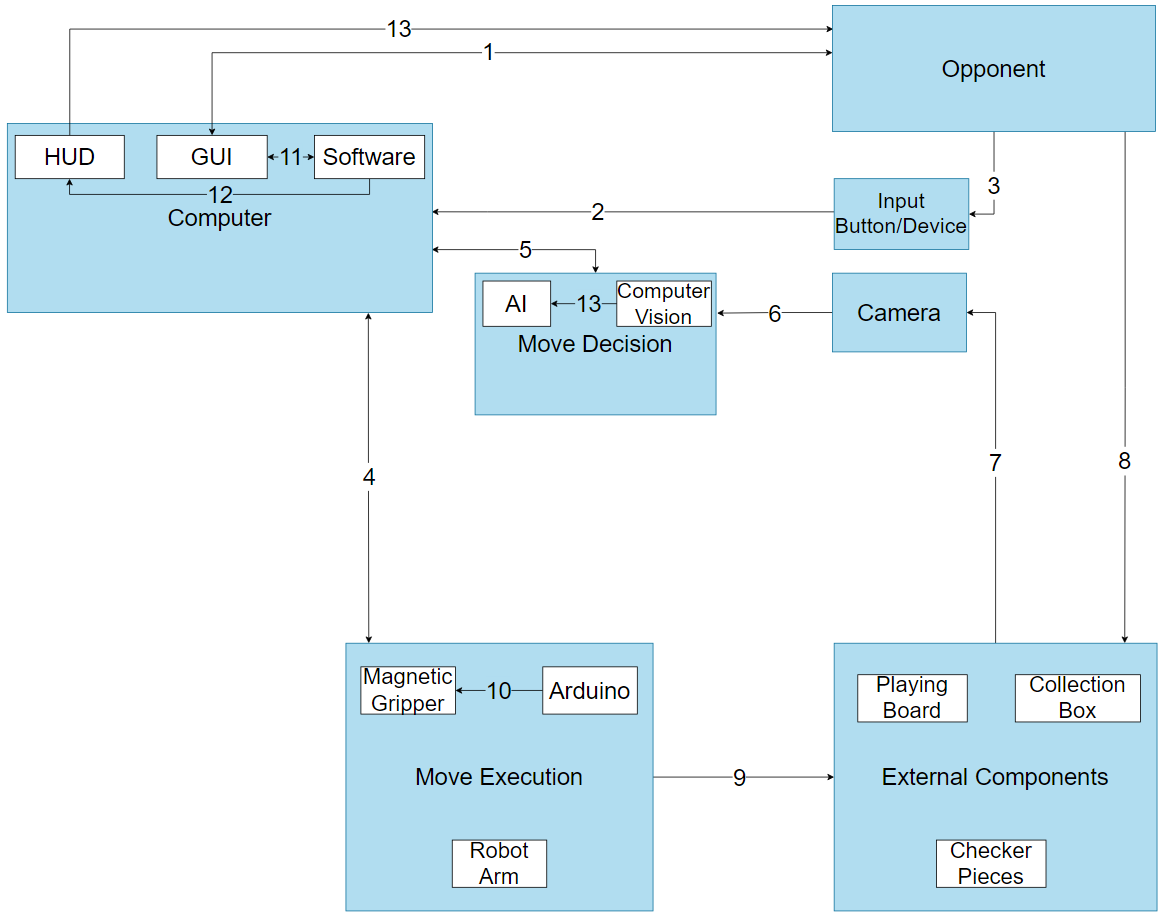
\includegraphics[width=0.90\textwidth]{images/data_flow_actual}
 \caption{System architecture}
\end{figure}

\section{Roles \& Responsibilities}
The stakeholders of the project are our course professor Dr. Christopher McMurrough and the University of Texas at Arlington since they will be investing in the production of this Checkers playing co-bot and will also be using the final product. Our point of contact from the customer side is Dr. Christopher McMurrough who is also our sponsor. Our point of contact from the developer side is Nimita Uprety. The team members are Nimita Uprety, Patricia Rojas, Hoang Ho, Kevin Vu, and Joanna Huynh. The roles and responsibilities of the team members are listed as follows which may change throughout the course of this project:\\

\textbf{1. Agile Roles:} \\The product owner will be Kevin Vu and the scrum master will be Patricia Rojas.\\

\textbf{2. Responsibilities:} \\The hardware technologies will be handled by Kevin Vu, Hoang Ho, Joanna Huynh, Patricia Rojas, and Nimita Uprety. Similarly, Computer Vision will be handled by Nimita Uprety, Hoang Ho, and Joanna Huynh. Additionally, Robotics will be handled by Kevin Vu, Hoang Ho, and Patricia Rojas. Finally, GUI will be handled by Nimita Uprety, Patricia Rojas, Joanna Huynh, and Kevin Vu.
\section{Cost Proposal}
The approximate budget of the project is 800 USD which will be dedicated towards buying a camera, suction cup, magnets, and other materials for the chess board and game. The camera will be necessary for the sensors to detect player movements, the suction cup for the gripper will be used in picking and placing Checkers, the magnet will be needed for sticking the Checkers pieces in place, the Checkers board will be made of birch plywood which will be bought and painted, the paint will be bought and used for the Checkers board, and the Checkers pieces will be 3D printed at the UT Arlington FabLab with the NinjaFlex Filament as the primary material. 

\subsection{Preliminary Budget}
\begin{table}[h]
\begin{center}
\begin{tabular}{ | m{12em} | m{10em}| m{10em} | } 
  \hline
  \textbf{Components} & \textbf{Quantity} & \textbf{Estimate(USD)} \\
  \hline
  Camera & 1 & 200 \\ 
  \hline
  Suction Cup & 1 & 50 \\ 
  \hline
  Magnets & 24 & 15 \\
  \hline
  Birch Plywood Panel (1/4 in. x 1.5 ft. x 1.5 ft.) & 1 & 20 \\ %for checkers board
  \hline
  Paint & 1 & 15 \\
  \hline
  3D Printed Checkers Pieces & 24 & 25 \\
  \hline
\end{tabular}
\caption{Preliminary Budget}
\end{center}
\end{table}
\subsection{Current \& Pending Support}
The default funding source for the project is the CSE Department who will provide 800 dollars for the project.
\section{Facilities \& Equipment}
% What lab space, testing grounds, makerspaces, etc. will you need to complete the project? Will you require any specific equipment, and if so, where will you get it (borrow, lease, purchase, outsource, already present in the lab, etc.). This section should occupy 1/2 page.

For our project we expect to be primarily utilizing the senior design lab facilities located in ERB 335 as this is where the UR5 Robot Arm should be stored throughout the majority of the year. This space will also be utilized by our team for the development, testing and implementation of any components we add to our project such as the camera and checker piece gripper. That said, the co-bot is currently being used on other projects and is not present in the senior design lab at the moment. The UR5 arm is expected to return to the ERB 335 lab soon but its final location is subject to change.

Given that our team is still undecided on what kind of gripper we will be implementing to pick up our checkers pieces we may or may not have an additional facility that we use. This is due to the fact that we are currently exploring two options, a vacuum gripper and an electropermanent magnetic one. If our team decides to make the gripper accessory magnetic, this means we will also need to 3D print our own checkers pieces so that we can put magnets inside them. In the event that we choose this option then we will utilize the available 3D printers in the FabLab to build our custom game pieces.

In terms of equipment the most vital piece is the UR5 Robot Arm itself. This piece will be leased from the College of Engineering at the University of Texas at Arlington. Additional equipment items include 3D printers (located in the FabLab) \& design software, Robot Operating Software [ROS]. However due to the complexity of our project this is not a final list of equipment pieces as we may need to use additional items to create our gripper accessories \& checkers pieces.

\section{Assumptions}
The following list contains critical assumptions related to the implementation and testing of the project:

\begin{itemize}
    \item Access to the UR5 Robot Arm will be available when needed for implementation and testing
    \item The UR5's controller box will be available and able to connect to a computer through an Ethernet cable
    \item A stable, large space with ample power, network connectivity, and enough lighting will be available for the project to reside in
    \item A gripper for the robot arm will be acquired by the 3rd sprint cycle
    \item A working camera for detection and sensing the game board will be acquired by the 3rd sprint cycle
\end{itemize}

% An assumption is a belief of what you assume to be true in the future. You make assumptions based on your knowledge, experience or the information available on hand. These are anticipated events or circumstances that are expected to occur during your project's life cycle.

% Assumptions are supposed to be true but do not necessarily end up being true. Sometimes they may turn out to be false, which can affect your project significantly. They add risks to the project because they may or may not be true. For example, if you are working on an outdoor unmanned vehicle, are you assuming that testing space will be available when needed? Are you relying on an external team or contractor to provide a certain subsystem on time? If you are working at a customer facility or deploying on their computing infrastructure, are you assuming you will be granted physical access or network credentials?

% This section should contain a list of at least 5 of the most critical assumptions related to your project. For example:

% The following list contains critical assumptions related to the implementation and testing of the project.

% \begin{itemize}
%   \item A suitable outdoor testing location will be available by the 3rd sprint cycle
%   \item The X sensing system developed by Sensor Consulting Company will be delivered according to specifications by the 4th sprint cycle
%   \item Access to the customer installation site will be provided by the 5th sprint cycle
%   \item The customer will provide ample power and network connectivity at the installation site
%   \item The installation site network infrastructure will allow TCP network traffic on port 8080
% \end{itemize}
\section{Constraints}
The following listed items are the projected constraints imposed on the checkers playing UR5 co-bot arm project:

\begin{itemize}
    \item The final prototype demonstration must be completed by May 1st, 2022.
    \item Total development costs for tools, hardware components, and 3D printing must not exceed \$800.
    \item The UR5 co-bot is located at a specific site, so access to it may be restricted by certain business hours. Additionally, programming and testing for robot is less flexible.
    \item Team members have minimal knowledge with computer vision and mechanical components, such as cameras, sensors, and grippers.
    \item Depending on the gripper type for the co-bot arm, a customized checkers board and pieces will have to be created.
    \item There is one co-bot arm for all members to work with.
    \item The UR5 co-bot may need specific lighting in the area that the checkers game is being played in order to adequately detect the pieces. 
    
\end{itemize}

% commented out the instructions using iffalse and fi
\iffalse
Constraints are limitations imposed on the project, such as the limitation of cost, schedule, or resources, and you have to work within the boundaries restricted by these constraints. All projects have constraints, which are defined and identified at the beginning of the project.

Constraints are outside of your control. They are imposed upon you by your client, organization, government regulations, availability of resources, etc. Occasionally, identified constraints turn out to be false. This is often beneficial to the development team, since it removes items that could potentially affect progress.

This section should contain a list of at least 5 of the most critical constraints related to your project. For example:

The following list contains key constraints related to the implementation and testing of the project.

\begin{itemize}
  \item Final prototype demonstration must be completed by May 1st, 20XX
  \item The customer will provide no more than two maintenance personnel to assist in on-site installation
  \item Customer installation site will only be accessible by development team during normal business hours
  \item Total development costs must not exceed \$800
  \item All data obtained from customer site must be reviewed and approved for release by the Information Security Office prior to being copied to any internet connected storage medium
\end{itemize}
\fi
\section{Risks}
% This section should contain a list of at least 5 of the most critical risks related to your project. Additionally, the probability of occurrence, size of loss, and risk exposure should be listed. For size of loss, express units as the number of days by which the project schedule would be delayed. For risk exposure, multiply the size of loss by the probability of occurrence to obtain the exposure in days. For example:

The following high-level risk census contains identified project risks with the highest exposure. Mitigation strategies will be discussed in future planning sessions.

\begin{table}[h]
\resizebox{\textwidth}{!}{
\begin{tabular}{|l|l|l|l|}
\hline
 \textbf{Risk description} & \textbf{Probability} & \textbf{Loss (days)} & \textbf{Exposure (days)} \\ \hline
 Availability of UR5 robot arm due to occupation on other projects  & 0.35 & 14 & 4.9 \\ \hline
 3D printed checkers pieces do not suction properly with robot & 0.40 & 9 & 3.6 \\ \hline
 UR5 robot arm out of commission due to broken components  & 0.25 & 14 & 3.5 \\ \hline
 Unexpected delays on shipping and delivery of parts & 0.10 & 20 & 2.0 \\ \hline
 Custom checkers playing board is incompatible in gameplay & 0.15 & 10 & 1.5 \\ \hline
\end{tabular}}
\caption{Overview of highest exposure project risks} 
\end{table}

% \begin{table}[h]
% \resizebox{\textwidth}{!}{
% \begin{tabular}{|l|l|l|l|}
% \hline
%  \textbf{Risk description} & \textbf{Probability} & \textbf{Loss (days)} & \textbf{Exposure (days)} \\ \hline
%  Availability of X sensor module due to contractor delay  & 0.50 & 20 & 10 \\ \hline
%  Outdoor testing grounds are not available  & 0.20 & 14 & 2.8 \\ \hline
%  Internet access not available at installation site  & 0.30 & 9 & 2.7 \\ \hline
%  Delays in shipping from overseas vendors  & 0.10 & 20 & 2.0 \\ \hline
%  Certification delays at compliance testing facility & 0.15 & 10 & 1.5 \\ \hline
% \end{tabular}}
% \caption{Overview of highest exposure project risks} 
% \end{table}
\section{Documentation \& Reporting}
%%% In this section, you will describe all of the various artifacts that you will generate and maintain during the project life cycle. Describe the purpose of each item below, how the content will be generated, where it will be stored, how often it will be updated, etc. Replace the default text for each section with your own description. Reword this paragraph as appropriate.

\subsection{Major Documentation Deliverables}
\subsubsection{Project Charter}
The project charter is intended to communicate Team UR5's understanding and research on the project. It is the current list of commitments the team will be making. The initial version of the document will be delivered October 3, 2022. The final version will be delivered during the second semester in May 2023. This document will be maintained and updated after every sprint as needed, and when the sponsor approves of these changes.

% Describe how this document will be maintained and updated (how often, under what circumstances, etc.). When will the initial version be delivered? When will the final version be delivered?
https://www.overleaf.com/project/631b8af69f1ea6c375d502b0
\subsubsection{System Requirements Specification}
The Systems Requirements Specification will be maintained and updated during every sprint as features are added or with further understanding of the technology. The initial version of this document will be delivered October 24, 2022. The final version will be delivered during the second semester in May 2023.

% Describe how this document will be maintained and updated (how often, under what circumstances, etc.). When will the initial version be delivered? When will the final version be delivered?

\subsubsection{Architectural Design Specification}
The Architectural Design Specification will be maintained and updated as needed during every sprint especially when there are changes in design or clarifications. The initial version of this document will be delivered November 14, 2022. The final version will be delivered during the second semester in May 2023.

% Describe how this document will be maintained and updated (how often, under what circumstances, etc.). When will the initial version be delivered? When will the final version be delivered?

\subsubsection{Detailed Design Specification}
The Detailed Design Specification will be maintained and updated as needed during every sprint especially when there are changes in design or clarifications. The initial version of this document will be delivered within the first quarter of 2023. The final version will be delivered during the second semester in May 2023.

% Describe how this document will be maintained and updated (how often, under what circumstances, etc.). When will the initial version be delivered? When will the final version be delivered?

\subsection{Recurring Sprint Items}
\subsubsection{Product Backlog}
Items will be added to the product backlog as the System Requirements Specification document is updated. These items will be prioritized based on customer needs and feasibility of the requirement for the current point in time. Team vote and feedback will also be taken into consideration. Jira Software by Atlassian will be used to maintain and work collaboratively on the product backlog.

% How will items be added to the product backlog from the SRS? How will these items be prioritized? Who makes the decision (product owner, group vote, etc.)? What software will be used to maintain and share the product backlog with team members and stakeholders?

\subsubsection{Sprint Planning}
Each sprint will be planned based on documentation and feature implementation deadlines. Team meetings will be held after each sprint to determine the sprint goals. There will be 4 sprints for the first semester and 4 sprints for the second semester, totalling 8 sprints for both semesters.

% How will each sprint plan be planned? How many sprints will there be (you need to look at the schedules for this course and previous Senior Design II courses during the appropriate semesters to figure this out).

\subsubsection{Sprint Goal}
The team will meet and discuss sprint goals. These sprint goals will be decide as a team. Our customer Christopher McMurrough will be involved in the process as needed through scheduled meetings.

% Who decides the sprint goal? How will you involve your customer in this process?

\subsubsection{Sprint Backlog}
Team discussion will be held to determine which product backlog items will make their way into the sprint backlog. The backlog will be maintained using Jira Software developed by Atlassian.

% Who decides which product backlog items make their way into the sprint backlog? How will the backlog be maintained (collaboration software, a "scrum board", etc.)?

\subsubsection{Task Breakdown}
Each team member will voluntarily claim a task, otherwise it will be random. Time spent on tasks will be documented using Jira Software.

% How will individual tasks be assigned from the sprint backlog? Will it be up to each team member to voluntarily claim a task, or will it come from the product owner? How will time spent on tasks be documented?

\subsubsection{Sprint Burn Down Charts}
The burn down charts will allow the team to track the progress of the project. Currently, using Jira Software will automatically generate the burn down charts for each sprint. Each individual team member is responsible for manually updating the effort and time spent as they complete each assigned task. Jira Software will also be able to access all of this. In addition to the Jira log, Microsoft Excel will be used to manually create the burn down charts in case members don't update on Jira. See Figure 2 and 3 for examples.

\begin{figure}[h!]
    \centering
    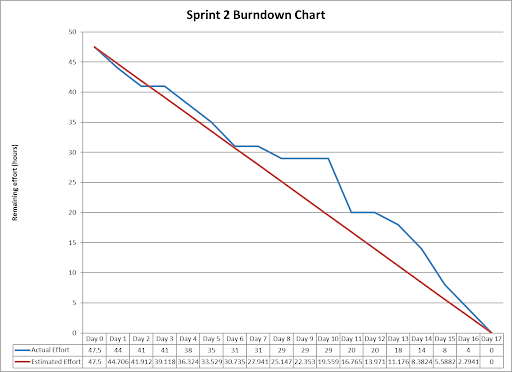
\includegraphics[width=1.0\textwidth]{images/burndown.png}
    \caption{Example sprint burn down chart}
\end{figure}

\begin{figure}[h!]
    \centering
    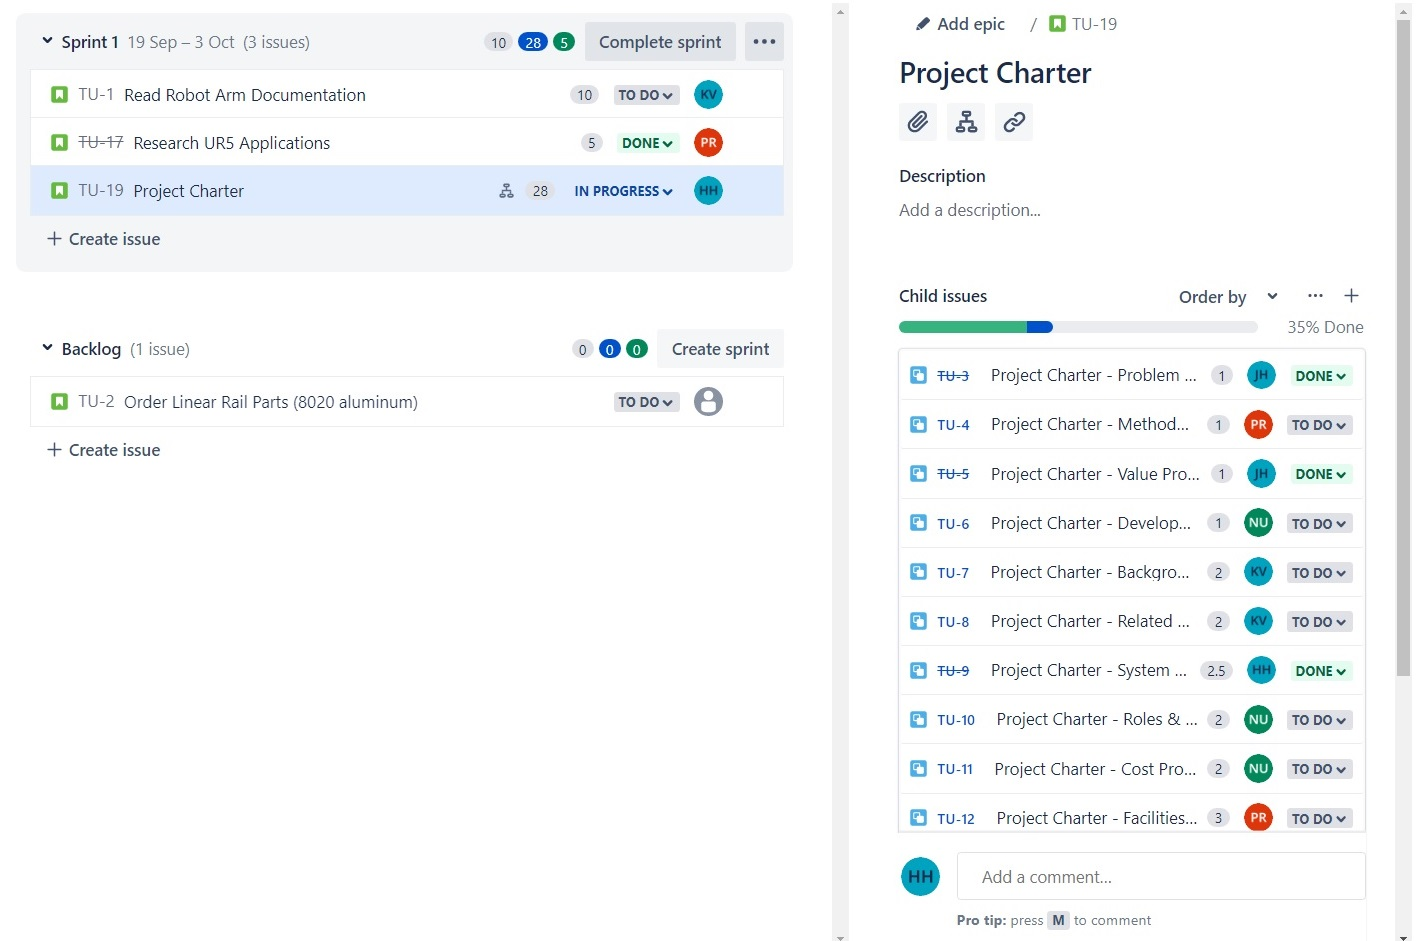
\includegraphics[width=1.0\textwidth]{images/sprint-burndown-tasks.jpg}
    \caption{Example task tracking}
\end{figure}

% Who will be responsible for generating the burn down charts for each sprint? How will they be able to access the total amount of effort expended by each individual team member? What format will the burn down chart use (include an example burn down chart below).

\subsubsection{Sprint Retrospective}
The sprint retrospective will be handled as a team during team meetings. This discussion will happen after each sprint review presentation at the end of each sprint. What went well, and what is needed to be adjusted will be documented as a team before the next sprint plan meeting.

% How will the sprint retrospective be handled as a team? When will this discussion happen after each sprint? What will be documented as a group and as individuals, and when will it be due?

\subsubsection{Individual Status Reports}
Each individual member will primarily report the tasks assigned to them and the time spent on each task for each sprint. Individuals can also include in their report any concerns or issues that may be addressed for future sprints.

% What sort of status will be reported by each individual member, and how often will it be reported? What key items will be contained in the report?

\subsubsection{Engineering Notebooks}
%%% notes, status reports, budgeting, sprint info
% The engineering notebook may contain any project notes, status reports, budgeting, sprint information, etc. It will be updated every week by each team member at minimum. The minimum amount of pages that will be completed will be 1 page for each sprint period. These sprint periods are around 2 weeks long. Any team member that is not the author will sign as a "witness" for each page.

% How often will the engineering notebook be updated, at a minimum, by each team member? What is the minimum amount of pages that will be completed for each interval, and how long will that interval be? How will the team keep each member accountable? Who will sign of as a "witness" for each ENB page?

\subsection{Closeout Materials}
\subsubsection{System Prototype}
Included in the final system prototype will be all major components (computer software, UR5, sensors, checkerboard, etc.) to demonstrate a game with the UR5.

% What will be included in the final system prototype? How and when will this be demonstrated? Will there be a Prototype Acceptance Test (PAT) with your customer? Will anything be demonstrated off-site? If so, will there be a Field Acceptance Test (FAT)?

\subsubsection{Project Poster}
Included on the project poster will be an overview, methodology and design, and results. Poster dimensions will be 32 inches tall by 40 inches wide.

% What will be included on the poster, what will be the final dimensions, and when will it be delivered?

% \subsubsection{Web Page}
% The project web page will have the project's overview, design, results, and document deliverables. The web page will be accessible to the public. When the web page will be delivered and updated is still to be decided.

% What will be included on the project web page? Will it be accessible to the public? When will this be delivered? Will it be updated throughout the project, or just provided at closeout (at a minimum, you need to provide a simple web page at the end).

\subsubsection{Demo Video}
Shown in the demo video will be the robot playing a game with a human. B-reel footage will be recorded throughout project implementation to show progress and different features.

% What will be shown in the demo video(s)? Will you include a B-reel footage for future video cuts? Approximately how long will the video(s) be, and what topics will be covered?

\subsubsection{Source Code}
The source code will be maintained on GitHub using the Git version control system. The source code will also be publicly available to the customer through GitHub. License terms are still to be decided, but still likely be listed in a single ReadMe file.

% How will your source code be maintained? What version control system will you adopt? Will source code be provided to the customer, or binaries only? If source code is provided, how will it be turned over to the customer? Will the project be open sourced to the general public? If so, what are the license terms (GNU, GPL, MIT, etc.). Where will the license terms be listed (in each source file, in a single readme file, etc.).

\subsubsection{Source Code Documentation}

The team plans to write a README for documentation and setup instructions for future users. The team also plans to potentially look into using Doxygen or Pydocs to generate the documentation. The format of the final documentation is still to be decided, however it is likely it will provided as a PDF or HTML file.

% The team plans to look into using Doxygen or Pydocs to generate the documentation. The format of the final documentation is still to be decided, however it is likely it will provided as a PDF or HTML file.

% What documentation standards will be employed? Will you use tools to generate the documentation (Doxygen, Javadocs, etc.). In what format will the final documentation be provided (PDF, browsable HTML, etc.)?

\subsubsection{Hardware Schematics}
The project will involve the UR5 Robot Arm. This robot arm will need a gripper for picking up pieces. In addition to that, a camera will be needed for the robot to detect the state of the game board, determine its next move, and move its pieces. The rest of the project involves python scripts.

% Will you be creating printed circuit boards (PCBs) or wiring components together? If so, list each applicable schematic and what sort of data it will contain (PCB layout, wiring diagram, etc.). If your project is purely software, omit this section.

\subsubsection{CAD files}
The project will need custom checker pieces if the UR5 plans to use a magnetic gripper to pick up the pieces. The FabLab at UTA has software support for SketchUp, Meshmixer, Tinkercad, Fusion 360, and SolidWorks. Currently, the plan is to use the free, online 3D modeling program Tinkercad to make the pieces. Blender could also be another free option to use outside of the software supported in the FabLab. The CAD files will be saved in STL file format to work with the 3D printers available in the FabLab at UTA.

% Will the project involve any mechanical design, such as 3D printed or laser-cut parts? If so, what software will you use to generate the files and what file formats will you provide in your closeout materials (STL, STEP, OBJ, etc.). If your project is purely software, omit this section.

\subsubsection{Installation Scripts}
There are currently no plans to provide installation scripts. At the moment, instructions are planned to be found in the ReadMe file on the GitHub repository.

% How will the customer deploy software to new installations? Will you provide installation scripts, install programs, or any other tools to improve the process? Will there be multiple scripts provided (perhaps separate scripts for the graphical front end and back end server software)? 

% \subsubsection{User Manual}
% A digital user manual will be provided for the customer. This digital user manual can also be printed.

% Will you customer need a printed or digital user manual? Will they need a setup video? Decide now what will be provided and discuss.
\newpage

%%% References
\bibliographystyle{plain}
\bibliographystyle{reference/IEEEtran_custom}
\bibliography{reference/refs}{}

\end{document}